\documentclass{article}

% Packages

% for floating graphics w/ captions
\usepackage{graphicx}
\usepackage{caption}
\usepackage{subcaption}
\usepackage{float}
\usepackage{listings}
\usepackage{color}

% links
\usepackage{hyperref}

% for math stuffs
\usepackage{amsmath}
\usepackage{amssymb}

% for ednotes
\usepackage[show]{ed}

% Other stuff
\usepackage{paralist}

% Unicode
\usepackage[utf8]{inputenc}
\DeclareUnicodeCharacter{00A0}{ }

% for citing
\usepackage[style=alphabetic]{biblatex}
\addbibresource{BDCCReport.bib}

\title{Establishing and Evaluating Access to Scientific Data \\ EUDAT Human Brain Project \\ Big Databases and Cloud Services \\ Project Report}
\author{Tom Wiesing}
\date{\today}

\definecolor{dkgreen}{rgb}{0,0.6,0}
\definecolor{gray}{rgb}{0.5,0.5,0.5}
\definecolor{mauve}{rgb}{0.58,0,0.82}

\lstset{frame=tb,
	language=Python,
	aboveskip=3mm,
	belowskip=3mm,
	showstringspaces=false,
	columns=flexible,
	basicstyle={\small\ttfamily},
	numbers=none,
	numberstyle=\tiny\color{gray},
	keywordstyle=\color{blue},
	commentstyle=\color{dkgreen},
	stringstyle=\color{mauve},
	breaklines=true,
	breakatwhitespace=true,
	tabsize=3
}

\begin{document}
	
	% Title Page
	\maketitle
	
	\ednote{Make an abstract}

	\newpage
	
	% Table of content
	\tableofcontents
	
	
	\vspace{\fill}\noindent	
	This work is licensed under the Creative Commons Attribution-NonCommercial-NoDerivatives 4.0 International License. To view a copy of this license, visit \url{http://creativecommons.org/licenses/by-nc-nd/4.0/} or send a letter to Creative Commons, PO Box 1866, Mountain View, CA 94042, USA. 
	\newpage
	
	% Section 1
	\section{Introduction}
	\label{sec:intro}

\subsection{Overview}

Multi-dimensional arrays arise naturally in multiple occasions and thus the paradigm of Array Databases has become more and more important. They can be used for a variety of scientific applications, ranging from satellite imagery, over medical imaging techniques to mathematically interesting objects.

One such array database is the Rasdaman system \cite{rasdaman:intropaper}. It promises to allow users to ``storing and querying massive multi-dimensional arrays, such as sensor, image, simulation, and statistics data appearing in domains like earth, space, and life science'' \cite{rasdaman:website}.

In this project we want to establish and evaluate access to scientific data. In particular we want to insert this scientific data into the Rasdaman database and evaluate how well the database can handle this kind of data. In this case we want to work together with EUDAT and the Human Brain Project.

\subsection{Collaborators}

The Human Brain Project \cite{hbp:website} is a European Commission Future and Emerging Technologies Flagship Project with the aim of ``providing research infrastructure in the fields of Neuroscience, computing and brain-related medicine''. In particular we collaborated with Huanxiang Lu and Dr. Sean Hill from the École polytechnique fédérale de Lausanne to gain access to the Human Brain Database. This archive of multiple sources is a database of (not only) human brain scans.

We also collaborated with Peter Wittenburg and Daan Broede from EUDAT \cite{eudat:website}. EUDAT is a ``collaborative Pan-European infrastructure for research data services, training and consultancy'' and will be used to host the data and resulting interfaces created in this project.

\subsection{Project Components}

Concretly this project consists of
\begin{inparaenum}[(1)]
\item gaining access to the scientific data provided by the Human Brain Database,
\item determining how (and if) this data can be represented inside the Rasdaman system,
\item developing a method to properly ingest the data into Rasdaman,
\item asking the collaborators about useful queries that can be performed on the data,
\item running the queries and gaining new insight into the data and finally
\item evaluating how well Rasdaman was able to deal with the provided data and developed queries.
\end{inparaenum}

The section of this report is as follows: In Section~\ref{sec:dataset} we introduce in detail the provided dataset. We then continue in Section~\ref{sec:ingestion} by describing how we ingested the data into Rasdaman. Next we describe the queries that we developed over the course of this project in Section~\ref{sec:queries} before coming to a short conclusion in Section~\ref{sec:outlook_conclusion}. 

	
	% Section 2
	\section{Human Brain Scans: The Dataset}
	\label{sec:dataset}

\subsection{The Human Brain Database Dataset}

The dataset we have worked with for this project comes from the Human Brain Database project. In total it is about 1 TB in size. It consists of a collection of different brain scans from different sources, each of different resolutions and shapes. Due to the size of this dataset we have not yet accessed all of it.

So far we have only worked with a small subset in order to test our methods. This subset is significantly smaller and is sourced from the SPM Anatomy toolbox \cite{SPMAnatomyToolbox:website}. It has a size of under 10 MB and is a brain atlas consisting of 27 different brain scans. Each scan has a resolution of about $150$ x $150$ x $200$ pixels.

\subsection{Neuroimaging Methods}

Before we describe the dataset in more detail we briefly introduce the reader to the most commonly used neuroimaging methods. This provides the neccessary background to understand what the data means. Neuroimaging is the process of scanning the brain and generating images of it. There are two different methods that are commonly used to achieve this.

X-ray computed tomography (commonly known as CT scan) is a method which produces multiple two-dimensional X-Ray images of an object to be scanned. With the help of computers these images are then assembled into a full three-dimensional scan. This allows to look inside an object without having to physically disassemble or open it.

Another common technique is called Magnetic resonance imaging and also known as an MRI scan. MRI scans do not use X-Rays to investigate an object but instead abuse the quantum spin of atoms. By applying a magnetic field, the spins of atoms are forced to align. Once this magnetic field is removed, the atoms return to equilibrium and produce very faint RF emissions. These can be detected, measured and then assembled into a three-dimensional image.

Both methods produce a 3-dimensional cube with scalar values at each point as the output, although MRI scans usually give higher resolution than X-Rays. For this reason our dataset consists mostly of MRI scans.

\subsection{The HDF Format And BBIC Encoding}

When we first received the dataset it was provided in HDF5 format. HDF stands for Hierarchical Data Format and is a data format that was originally developed at National Center for Supercomputing Applications  and is now mainted by the HDF Group \cite{HDF5:website}. It is designed to store and organize large amounts of data and has two different kinds of objects, datasets and groups. Datasets are multi-dimensional arrays of homogeneous type. Groups are containers for datasets and sub groups. This results in a filesystem-like structure for HDF5 files.

Even though the data is stored inside an HDF file, it is encoded using the BBIC format. This is an internal format used mostly for an image viewer by our collaborators. Our collaborators stated that ``the bbic format contains a stack of tiled images of different level/resolution. Our image viewer works just like the Google Maps. Every time we zoom in or out, the viewer sends a query to the image service to retrieve certain tiles of images of certain slice at certain resolution'' \cite{BBIC:about}. This makes it very difficult for us to extract the original three-dimensional cube that represents the brain scan. What makes it even more difficult is the fact that there is very little documentation available because the  ``bbic format was developed by a former colleague who has left for long time before I joined'' \cite{BBIC:dev}.

\subsection{The ATLAS Viewer}

The BBIC format is used for the so-called ATLAS viewer. It is based on the imaging service mentioned above and is available at \cite{hbp:atlasviewer}. The viewer allows the user to interactively explore a subset of the Human Brain Database.

The atlas viewer has three main features:
\begin{inparaenum}[(1)]
\item selection of different brain scans,
\item looking at different two-dimensional cuts through the original data (Figure~\ref{fig:atlas_browser}) and
\item overlaying of brain region masks (Figure~\ref{fig:atlas_masks}).
\end{inparaenum}

\begin{figure}[h]
\centering
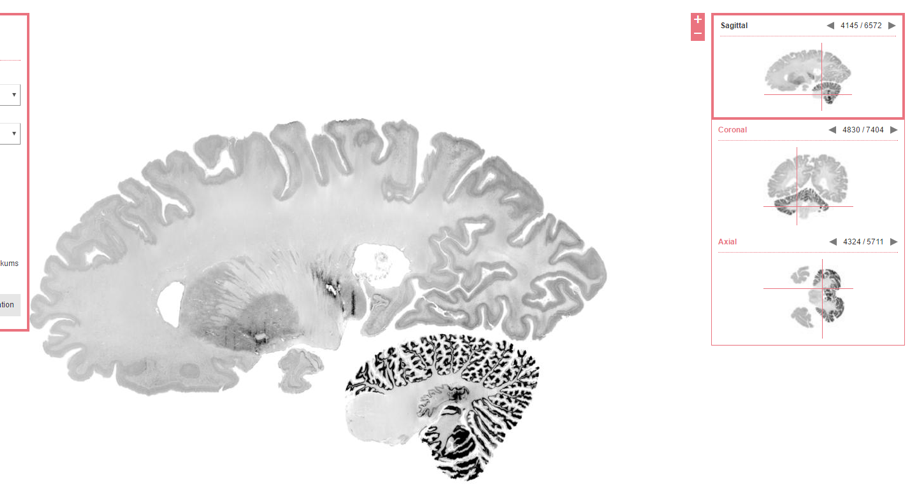
\includegraphics[width=\textwidth]{imgs/atlas_browse}
\caption{A screenshot of the ATLAS viewer showing a basic cut through a single dataset. }
\label{fig:atlas_browser}
\end{figure}

\begin{figure}[h]
\centering
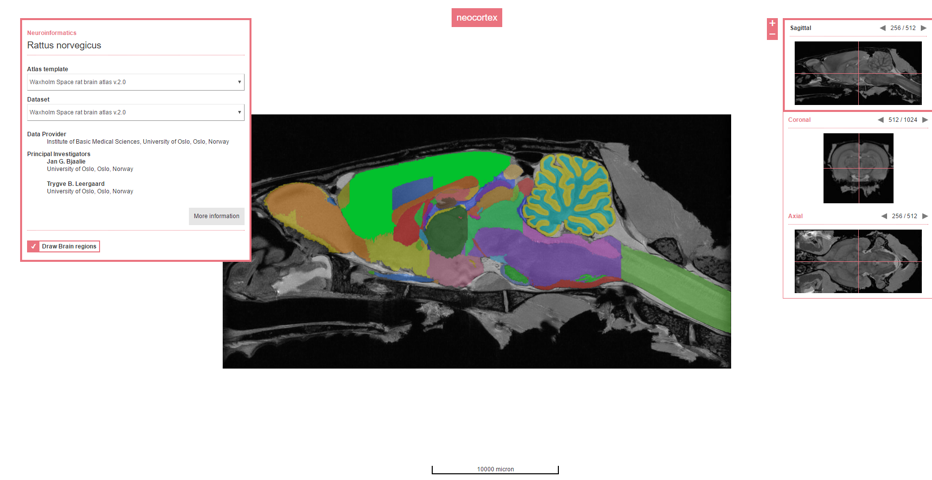
\includegraphics[width=\textwidth]{imgs/atlas_masks}
\caption{A screenshot of the ATLAS viewer showing an overlayed brain region mask. }
\label{fig:atlas_masks}
\end{figure}

	
	% Section 3
	\section{Data Ingestion}
	\label{sec:ingestion}
\ednote{Write this}
	
	% Section 4
	\section{Querying the Dataset}
	\label{sec:queries}

\subsection{Slicing An Image Cube}

Now that the data has been ingested into Rasdaman we proceeded with writing simple queries. Since Rasdaman is an Array Database system which has been used for multi-dimensional data we first wanted to start this part of the project by reproducing the functionaility of the ATLAS viewer described above. For this we want to start with simple slicing operations, namely just extracting Sagittal, Coronal and Axial\footnote{Sagittal, Coronal and Axial cuts are domain specific terms for cuts parallel to the axes of the data cube. } slices from the original scan.

Rasdaman is capable of expressing these cuts easily. Each of them is parameterized by two parameters, the two axes it is parallel to and the position within the third axis where to cut. In the query language this uses a slicing operation and is written as \lstinline[morekeywords={NAME,INDEX},language=SQL]{select it[INDEX,*:*,*:*] from NAME as it}. Here \lstinline{INDEX} refers to the position of where to cut and \lstinline{NAME} refers to the name of the collection that contains the data cube.

\begin{figure}[h]
\centering
\begin{subfigure}{.3\textwidth}
  \centering
  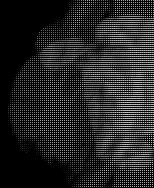
\includegraphics[width=\textwidth]{imgs/CutA}
\end{subfigure}%
\space\space\space
\begin{subfigure}{.3\textwidth}
  \centering
  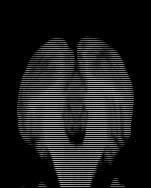
\includegraphics[width=\textwidth]{imgs/CutB}
\end{subfigure}
\space\space\space
\begin{subfigure}{.3\textwidth}
  \centering
  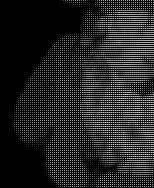
\includegraphics[width=\textwidth]{imgs/CutC}
\end{subfigure}
\caption{Simple cuts through the example dataset. }
\label{fig:cuts}
\end{figure}

Additionally in order to display the output from this operation we need to choose an image format to display it in. To save such a cut as a png image a command like
\begin{lstlisting}[showstringspaces=false,morekeywords={NAME,INDEX,FILENAME},language=Bash]
rasql -q "select encode(it[INDEX,*:*,*:*],\"png\") from NAME as it" --out file --outfile FILENAME
\end{lstlisting}
can be used. A sample output of this operation can be found in Figure~\ref{fig:cuts}.

\subsection{Overlaying Brain Region Masks}

The second operation of the ATLAS viewer that is interesting to reproduce is the overlaying of Brain Region Masks onto the original scan. This operation is more complicated than the simple slicing operation and any query performing it needs to perform the following three steps:
\begin{enumerate}
  \item retrieve the brain scan data
  \item retrieve the brain mask data
  \item overlay the mask over the brain data
\end{enumerate}

A command similar to the following could be used to produce a single Brain region mask overlay:
\begin{lstlisting}[showstringspaces=false,morekeywords={INDEX,MASK_COLLECTION,SCAN_COLLECTION,FILENAME},language=Bash]
rasql -q "select encode(S[INDEX,*:*,*:*] overlay M[INDEX,*:*,*:*], \"png\") from MASK_COLLECTION M, SCAN_COLLECTION S" --out file --filename FILENAME
\end{lstlisting}

In this command we assume that the brain scan data and the mask data are available in the collections \lstinline{SCAN_COLLECTION} and \lstinline{MASK_COLLECTION} respctively. Then we use the \lstinline{overlay} operator to overlay the two images.

\begin{figure}[h]
  \centering
  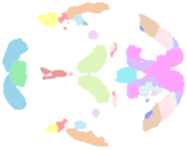
\includegraphics{imgs/Mask}
  \caption{Example Brain Mask Data}
  \label{fig:mask}
\end{figure}

In practive the second step of retrieve brain mask data provides significant difficulties. Even though the brain mask data is available in principal it is only given in the form of an SVG image. Unlike the brain scan data, this is a vector image format which does not store the rasterized representation as would be needed by Rasdaman. On top of this the SVG images do not contain three-dimensional data but are instead structured similar to the BBIC format. For each possible cut and zoom level a seperate image is provided. One of these image can be found in Figure~\ref{fig:mask}. Unfortunatly these problems stopped us from properly ingesting the brain mask data into Rasdaman.

\subsection{Extended Slices}

The final type of query we wanted to experiment with expands on the slicing explained above. Instead of only allowing cuts parallel to two of the three axes we wanted to allow any type of two-dimensional cuts. While this is not available in the ATLAS viewer it is an enhancement our collaborators have been thinking about. Mathematically speaking such a cut consists of an arbitrary two-dimensional plane intersecting a three-dimensional cuboid. As such it is parametrised by 6 parameters, one (three-dimensional) point to start the plane at and three angles in each direction to rotate the plane along.

This mathematical description gives us one natural way to represent this query inside Rasdaman: Rotate the entire cube according to the three angles given above and then perform a simple cut as described above. Unfortunatly there is no rotation operation inside Rasdaman, but according to \cite{rasdaman:issue228} it might be added in the future.

There is a second way to represent these queries inside Rasdaman. Outside of Rasdaman one can compute the coordinates that would be included in the plane and then query the database for those exact values. Even though this could be simplified by using arrays to index the data cube, this still requires some non-trivial computational effort outside of Rasdaman and thus we did not perform this query either.

		
	% Section 5
	\section{Outlook \& Conclusion}
	\label{sec:outlook_conclusion}

In this project we have collaborated with Human Brain Database researchers. We have looked at their data and modelled this inside Rasdaman. We have written a script to automatically ingest more data in the future. We also investigated which queries are of use and implemented a few basic queries inside our database.

The research in this direction is far from complete however. With the work we have achieved we have provided a base line for reproducing the functionality of the ATLAS viewer and future projects should be able to build on this. Even though the provided queries allow users to investigate the data set as is, an interface should be implemented on top of this so that users without database knowledge can also interact with the dataset.

Furthermore the methods described in this report have only been tested with a small fraction of the dataset and most of it has yet to be ingested. A further direction worth researching might also include generating the brain region masks provided automatically. Such a project would likely involve a Machine Learning component.

	
	\printbibliography
\end{document}